% Created by tikzDevice version 0.12.6 on 2026-05-14 21:46:45
% !TEX encoding = UTF-8 Unicode
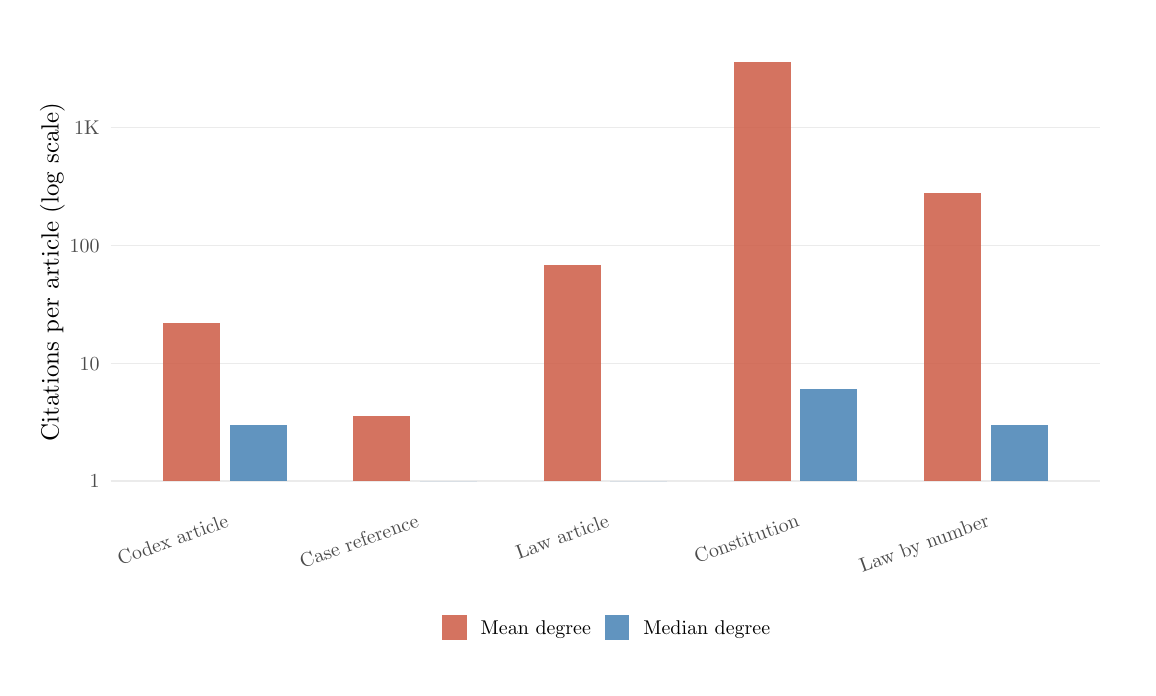
\begin{tikzpicture}[x=1pt,y=1pt]
\definecolor{fillColor}{RGB}{255,255,255}
\path[use as bounding box,fill=fillColor,fill opacity=0.00] (0,0) rectangle (397.48,231.26);
\begin{scope}
\path[clip] (  0.00,  0.00) rectangle (397.48,231.26);
\definecolor{fillColor}{RGB}{255,255,255}

\path[fill=fillColor] ( -0.00,  0.00) rectangle (397.48,231.26);
\end{scope}
\begin{scope}
\path[clip] ( 30.05, 59.85) rectangle (387.48,226.26);
\definecolor{drawColor}{gray}{0.92}

\path[draw=drawColor,line width= 0.5pt,line join=round] ( 30.05, 67.41) --
	(387.48, 67.41);

\path[draw=drawColor,line width= 0.5pt,line join=round] ( 30.05,110.00) --
	(387.48,110.00);

\path[draw=drawColor,line width= 0.5pt,line join=round] ( 30.05,152.58) --
	(387.48,152.58);

\path[draw=drawColor,line width= 0.5pt,line join=round] ( 30.05,195.17) --
	(387.48,195.17);
\definecolor{fillColor}{RGB}{70,130,180}

\path[fill=fillColor,fill opacity=0.85] ( 73.01, 67.41) rectangle ( 93.63, 87.73);

\path[fill=fillColor,fill opacity=0.85] (141.75, 67.41) rectangle (162.37, 67.41);

\path[fill=fillColor,fill opacity=0.85] (210.48, 67.41) rectangle (231.11, 67.41);

\path[fill=fillColor,fill opacity=0.85] (279.22, 67.41) rectangle (299.84,100.55);

\path[fill=fillColor,fill opacity=0.85] (347.96, 67.41) rectangle (368.58, 87.73);
\definecolor{fillColor}{RGB}{205,91,69}

\path[fill=fillColor,fill opacity=0.85] ( 48.95, 67.41) rectangle ( 69.57,124.58);

\path[fill=fillColor,fill opacity=0.85] (117.69, 67.41) rectangle (138.31, 91.10);

\path[fill=fillColor,fill opacity=0.85] (186.43, 67.41) rectangle (207.05,145.48);

\path[fill=fillColor,fill opacity=0.85] (255.16, 67.41) rectangle (275.79,218.70);

\path[fill=fillColor,fill opacity=0.85] (323.90, 67.41) rectangle (344.52,171.52);
\end{scope}
\begin{scope}
\path[clip] (  0.00,  0.00) rectangle (397.48,231.26);
\definecolor{drawColor}{gray}{0.30}

\node[text=drawColor,anchor=base east,inner sep=0pt, outer sep=0pt, scale=  0.72] at ( 26.00, 64.93) {1};

\node[text=drawColor,anchor=base east,inner sep=0pt, outer sep=0pt, scale=  0.72] at ( 26.00,107.52) {10};

\node[text=drawColor,anchor=base east,inner sep=0pt, outer sep=0pt, scale=  0.72] at ( 26.00,150.10) {100};

\node[text=drawColor,anchor=base east,inner sep=0pt, outer sep=0pt, scale=  0.72] at ( 26.00,192.69) {1K};
\end{scope}
\begin{scope}
\path[clip] (  0.00,  0.00) rectangle (397.48,231.26);
\definecolor{drawColor}{gray}{0.30}

\node[text=drawColor,rotate= 20.00,anchor=base east,inner sep=0pt, outer sep=0pt, scale=  0.72] at ( 72.98, 51.14) {Codex article};

\node[text=drawColor,rotate= 20.00,anchor=base east,inner sep=0pt, outer sep=0pt, scale=  0.72] at (141.72, 51.14) {Case reference};

\node[text=drawColor,rotate= 20.00,anchor=base east,inner sep=0pt, outer sep=0pt, scale=  0.72] at (210.46, 51.14) {Law article};

\node[text=drawColor,rotate= 20.00,anchor=base east,inner sep=0pt, outer sep=0pt, scale=  0.72] at (279.20, 51.14) {Constitution};

\node[text=drawColor,rotate= 20.00,anchor=base east,inner sep=0pt, outer sep=0pt, scale=  0.72] at (347.94, 51.14) {Law by number};
\end{scope}
\begin{scope}
\path[clip] (  0.00,  0.00) rectangle (397.48,231.26);
\definecolor{drawColor}{RGB}{0,0,0}

\node[text=drawColor,rotate= 90.00,anchor=base,inner sep=0pt, outer sep=0pt, scale=  0.90] at ( 11.20,143.06) {Citations per article (log scale)};
\end{scope}
\begin{scope}
\path[clip] (  0.00,  0.00) rectangle (397.48,231.26);
\definecolor{fillColor}{RGB}{205,91,69}

\path[fill=fillColor,fill opacity=0.85] (149.83, 10.08) rectangle (158.62, 18.88);
\end{scope}
\begin{scope}
\path[clip] (  0.00,  0.00) rectangle (397.48,231.26);
\definecolor{fillColor}{RGB}{70,130,180}

\path[fill=fillColor,fill opacity=0.85] (208.60, 10.08) rectangle (217.39, 18.88);
\end{scope}
\begin{scope}
\path[clip] (  0.00,  0.00) rectangle (397.48,231.26);
\definecolor{drawColor}{RGB}{0,0,0}

\node[text=drawColor,anchor=base west,inner sep=0pt, outer sep=0pt, scale=  0.72] at (163.71, 12.00) {Mean degree};
\end{scope}
\begin{scope}
\path[clip] (  0.00,  0.00) rectangle (397.48,231.26);
\definecolor{drawColor}{RGB}{0,0,0}

\node[text=drawColor,anchor=base west,inner sep=0pt, outer sep=0pt, scale=  0.72] at (222.47, 12.00) {Median degree};
\end{scope}
\end{tikzpicture}
